\section{4-component graph}
An experiment with synthetic data generated by a 4-component graph was conducted.
We consider the following model:
\begin{equation}
  \mathbf{L}_{\mathsf{noisy}} = \mathbf{L}_{\mathsf{true}} + \mathbf{L}_{\mathsf{ER}},
  \label{eq:model}
\end{equation}
where $\mathbf{L}_{\mathsf{true}}$ represents the Laplacian matrix of a $K$-component graph (for this example, $K = 4$)
denoted as $\mathcal{G}^{(p_1, p_2)}_K$,
in which $p_1$ and $p_2$ represent the probabilities of node connections across components and within components, respectively;
$\mathbf{L}_{\mathsf{ER}}$ represents the Laplacian of an Erdos-Renyi graph $\mathcal{G}^{(p)}_{\mathsf{ER}}$, in which $p$
is the probability of a node connecting to any other node. The weighted edges of $\mathcal{G}^{(p_1, p_2)}_K$
were drawn from $\textsf{Uniform}(0, 1)$, whereas the ones of $\mathcal{G}^{(p)}_{\mathsf{ER}}$ where drawn from
$\textsf{Uniform}(0, \kappa)$, in which $\kappa \in (0, 1)$ controls how much noise is added to the true graph. Finally,
we set $p_1 = 0$, $p_2 = 1$, $p = 0.35$, and $\kappa = 0.45$.

Then, data were sampled in the form of $\mathbf{Y} \thicksim \mathcal{N}(\mathbf{0}, \mathbf{L}_{\mathsf{noisy}}^{\dagger})$,
where $\mathbf{A}^{\dagger}$ denotes the generalized inverse of the matrix $\mathbf{A}$. The total number of nodes $N$
and the number of drawn samples $T$ were set to $N = 20$ (5 nodes per component) and $T / N = 30$.

Figure~\ref{fig:4-comp} illustrates the ground truth model, its noisy version, and the model learned by our spectral
topology algorithm with $\beta = 20 \cdot N$ and $\alpha = 0.1$.
We compute the performance of the learning process by means of the relative error
($\textsf{RE}$) and the F-score ($\textsf{FS}$). For this example, our algorithm achives $(\mathsf{RE}, \mathsf{FS}) = (0.210, 1)$
which means a perfect clustering accuracy even in a noisy model that heavily suppress the ground truth weights.

\begin{figure}[!htb]
    \centering
    \begin{subfigure}[b]{0.3\textwidth}
      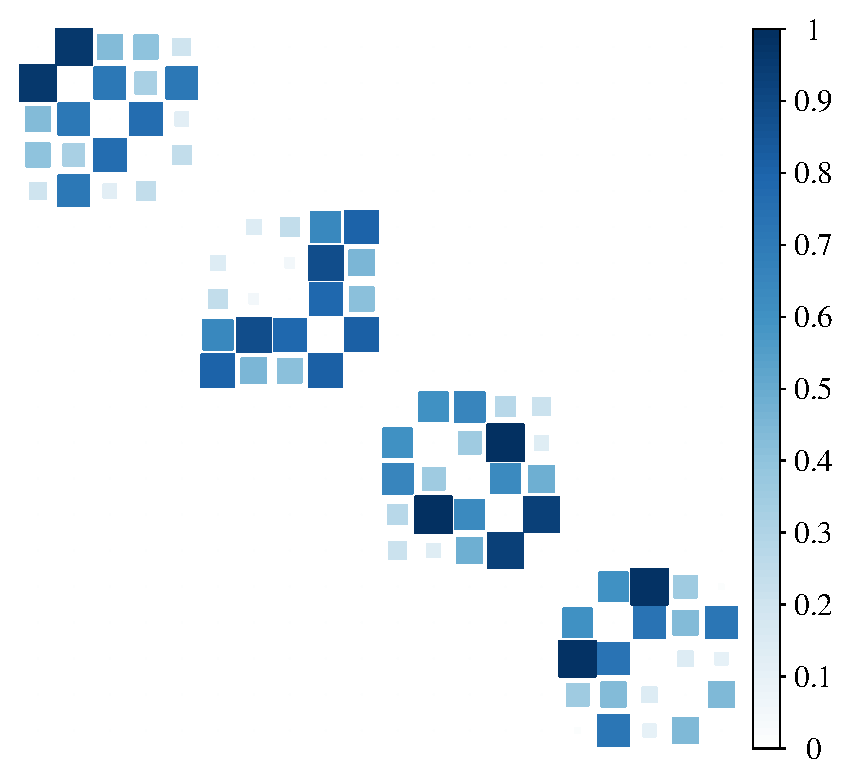
\includegraphics[width=\textwidth]{block-diagonal/latex/figures/true_mat.eps}
        \caption{Ground Truth Laplacian matrix}
    \end{subfigure}
    ~ %add desired spacing between images, e. g. ~, \quad, \qquad, \hfill etc.
      %(or a blank line to force the subfigure onto a new line)
    \begin{subfigure}[b]{0.3\textwidth}
        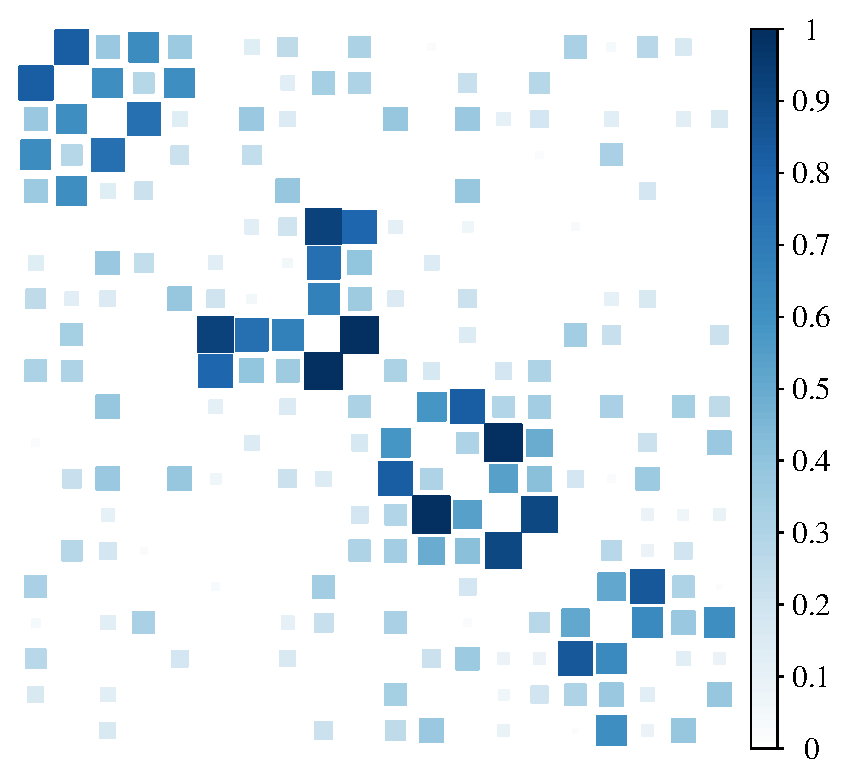
\includegraphics[width=\textwidth]{block-diagonal/latex/figures/noisy_mat.eps}
        \caption{Noisy Laplacian matrix}
    \end{subfigure}
    ~ %add desired spacing between images, e. g. ~, \quad, \qquad, \hfill etc.
    %(or a blank line to force the subfigure onto a new line)
    \begin{subfigure}[b]{0.3\textwidth}
        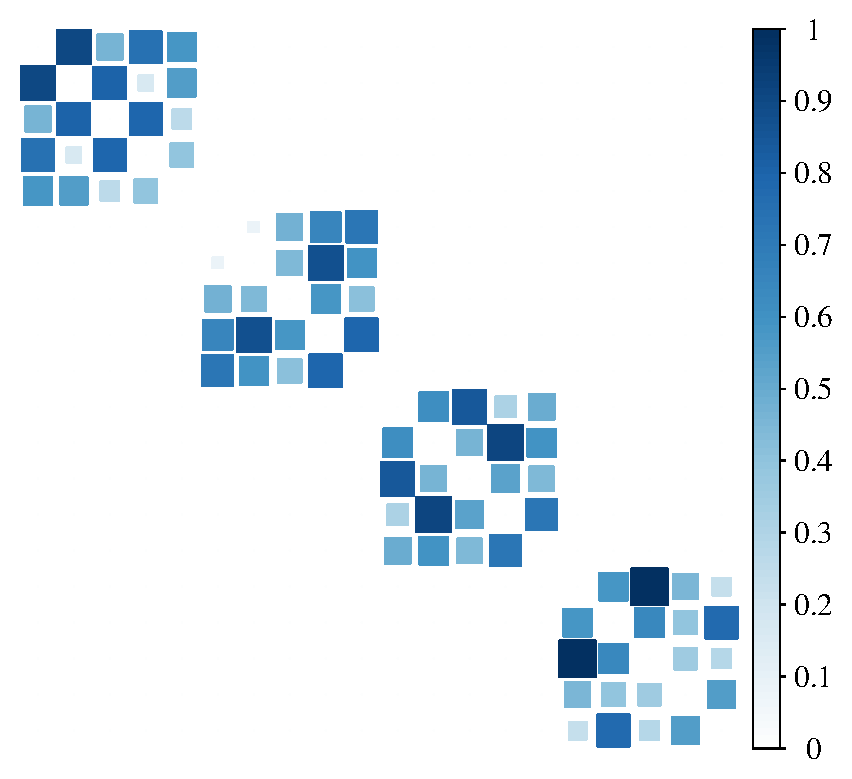
\includegraphics[width=\textwidth]{block-diagonal/latex/figures/est_mat.eps}
        \caption{Learned Laplacian matrix}
    \end{subfigure}
        \\
    \begin{subfigure}[b]{0.3\textwidth}
        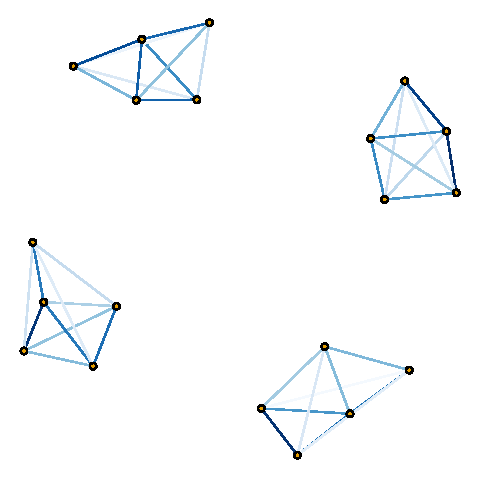
\includegraphics[width=\textwidth]{block-diagonal/latex/figures/true_graph.eps}
        \caption{Ground Truth graph}
    \end{subfigure}
    ~ %add desired spacing between images, e. g. ~, \quad, \qquad, \hfill etc.
      %(or a blank line to force the subfigure onto a new line)
    \begin{subfigure}[b]{0.3\textwidth}
        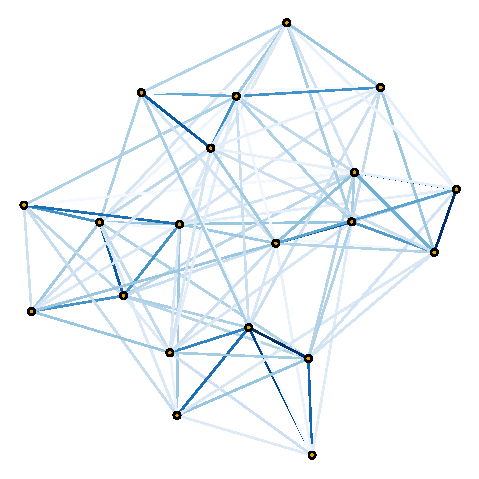
\includegraphics[width=\textwidth]{block-diagonal/latex/figures/noisy_graph.eps}
        \caption{Noisy graph}
    \end{subfigure}
    ~ %add desired spacing between images, e. g. ~, \quad, \qquad, \hfill etc.
    %(or a blank line to force the subfigure onto a new line)
    \begin{subfigure}[b]{0.3\textwidth}
        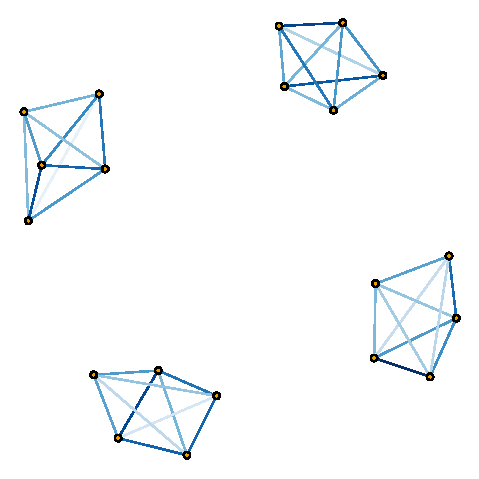
\includegraphics[width=\textwidth]{block-diagonal/latex/figures/est_graph.eps}
            \caption{Learned graph}
    \end{subfigure}
        \caption{An example of estimating a 4-component graph. (a) the ground truth graph Laplacian matrix ($\mathbf{L}_{\mathsf{true}}$),
                 (b) $\mathbf{L}_{\mathsf{true}}$ after being corrupted by noise, (c) the learned graph Laplacian with a performance of
                 $(\mathsf{RE}, \mathsf{FS}) = (0.210, 1)$.
                 The panels (d), (e), and (f) correspond to the graphs represented by the Laplacian matrices in
                 (a), (b), and (c), respectively.}\label{fig:4-comp-graph}
        \label{fig:4-comp}
\end{figure}

Figure~\ref{fig:performance} shows the performance of our algorithm, using the same settings as the experiment above,
but for different noise regimes.
\begin{figure}[!htb]
    \begin{subfigure}[b]{0.45\textwidth}
        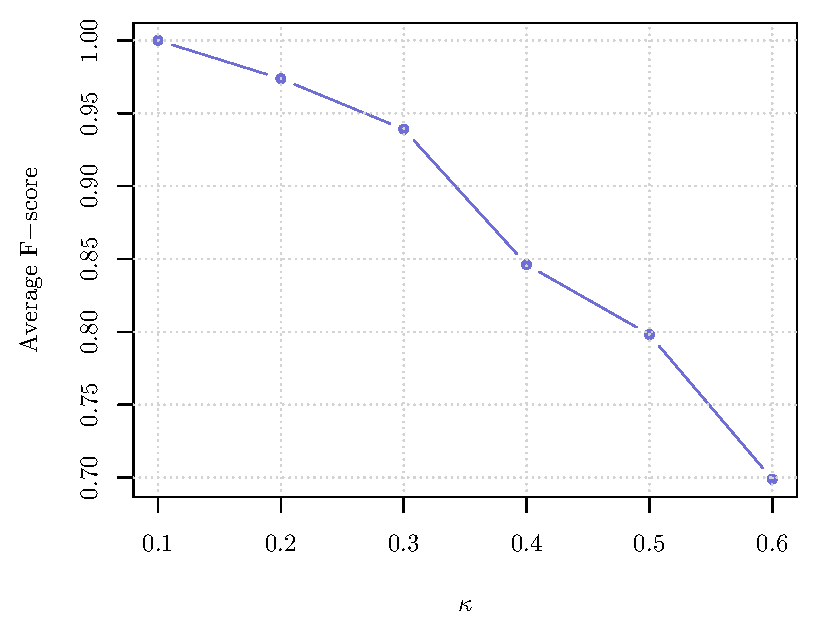
\includegraphics[width=\textwidth]{block-diagonal/latex/figures/fscore_kappa.eps}
        \caption{Average F-score vs noise factor}
    \end{subfigure}
    \begin{subfigure}[b]{0.45\textwidth}
        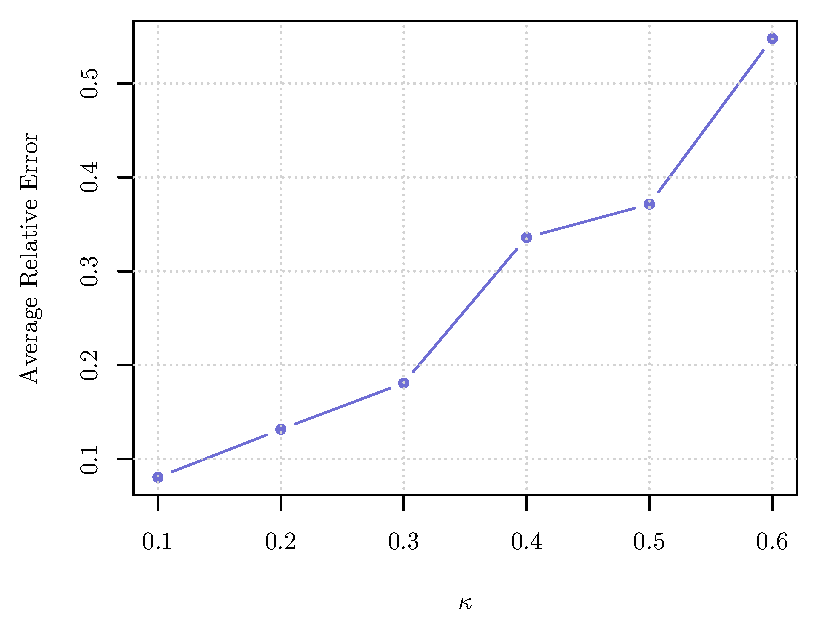
\includegraphics[width=\textwidth]{block-diagonal/latex/figures/relative_error_kappa.eps}
        \caption{Relative error vs noise factor}
    \end{subfigure}
    \caption{Average performance results, as a function of the noise factor, for learning Laplacian matrix of a modular graph embedded in noise.}
    \label{fig:performance}
\end{figure}

\section{Performance}
To infer the performance as a function of the ratio $T/N$, we consider a 4-component graph in which every component has
four nodes connected with probability 1. The edge weights among nodes are drawn from \text{Uniform}(0.1, 3). Additionally,
we perform a grid search on the sparsity parameter $\alpha$, just like the one performed by Elgimez.

\begin{figure}[!htb]
  \begin{subfigure}[b]{0.45\textwidth}
      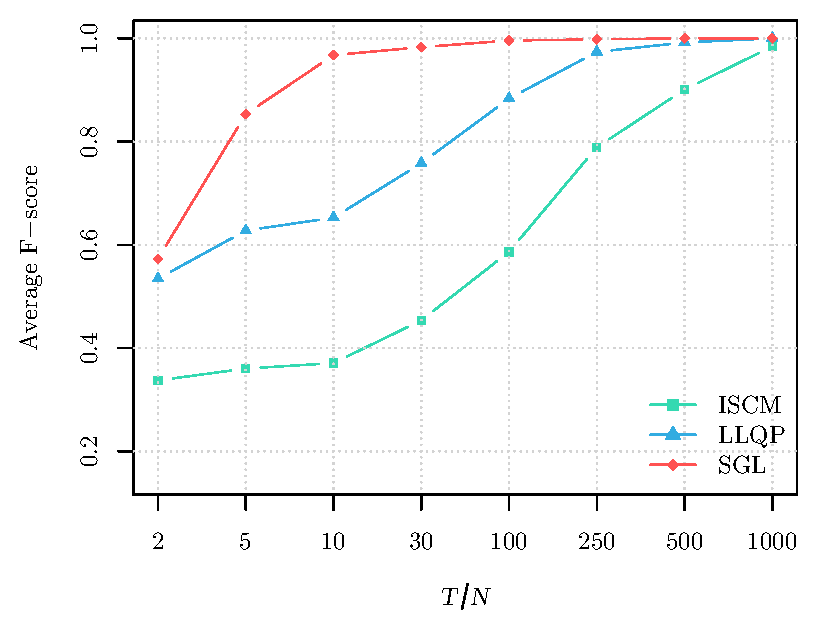
\includegraphics[width=\textwidth]{block-diagonal/latex/figures/fscore_block_diagonal.eps}
      \caption{Average F-score vs $T/N$}
  \end{subfigure}
  \begin{subfigure}[b]{0.45\textwidth}
      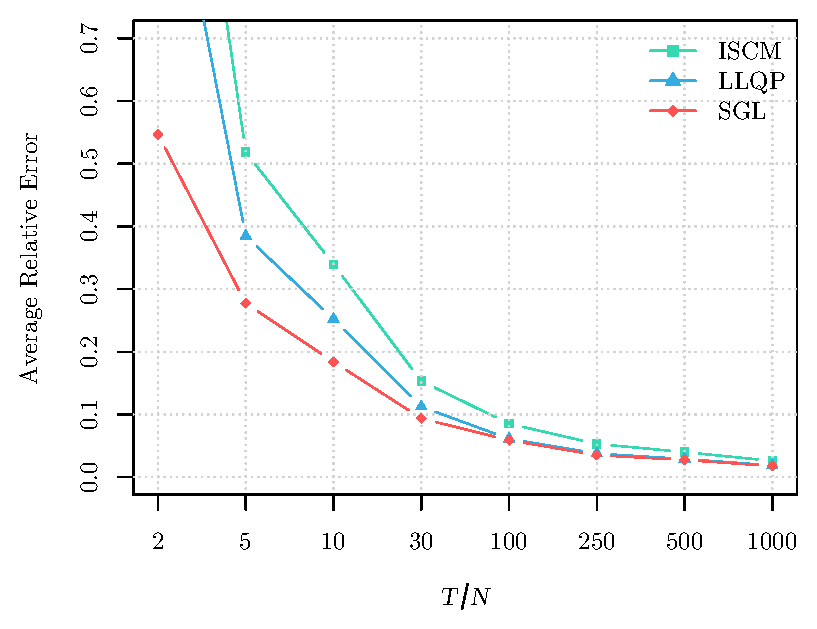
\includegraphics[width=\textwidth]{block-diagonal/latex/figures/relative_error_block_diagonal.eps}
      \caption{Average Relative Error vs $T/N$}
  \end{subfigure}
  \caption{Average performance results as, a function of the number of samples, for learning
           Laplacian matrix of a 4-component graph.}
  \label{fig:performance}
\end{figure}
